\documentclass[10pt,DIV16,a4paper,abstract=true,twoside=semi,openright]
{scrreprt}
\usepackage[USenglish]{babel}
\usepackage[numbers, sort&compress]{natbib}
\usepackage{isabelle,isabellesym}
\usepackage{booktabs}
\usepackage{paralist}
\usepackage{graphicx}
\usepackage{amssymb}
\usepackage{xspace}
\usepackage{xcolor}
\usepackage{listings}
\lstloadlanguages{HTML}
\usepackage[]{mathtools}
\usepackage[pdfpagelabels, pageanchor=false, plainpages=false]{hyperref}
\lstdefinestyle{html}{language=XML,
  basicstyle=\ttfamily,
  commentstyle=\itshape,
  keywordstyle=\color{blue},
  ndkeywordstyle=\color{blue},
}
\lstdefinestyle{displayhtml}{style=html,
  floatplacement={tbp},
  captionpos=b,
  framexleftmargin=0pt,
  basicstyle=\ttfamily\scriptsize,
  backgroundcolor=\color{black!2},
  frame=lines,
}
\lstnewenvironment{html}[1][]{\lstset{style=displayhtml, #1}}{}
\def\inlinehtml{\lstinline[style=html, columns=fullflexible]}
 \newsavebox{\fstlst}
  \newsavebox{\sndlst}
\usepackage[caption=false]{subfig}

\pagestyle{headings}
\isabellestyle{default}
\setcounter{tocdepth}{1}
\newcommand{\ie}{i.\,e.\xspace}
\newcommand{\eg}{e.\,g.\xspace}
\newcommand{\thy}{\isabellecontext}
\renewcommand{\isamarkupsection}[1]{%
  \begingroup% 
  \def\isacharunderscore{\textunderscore}%
  \section{#1 (\thy)}%
  \endgroup% 
}

\title{A Formalization of Web Components} 
\author{Achim~D.~Brucker \and Michael~Herzberg}%
\publishers{
  \footnotemark[1]~Department of Computer Science, University of Exeter, Exeter, UK\texorpdfstring{\\}{, }
  \texttt{a.brucker@exeter.ac.uk}\\[2em]
  %
  \footnotemark[2]~  Department of Computer Science, The University of Sheffield, Sheffield, UK\texorpdfstring{\\}{, }
   \texttt{msherzberg1@sheffield.ac.uk}
}
\begin{document}
  \maketitle
  \begin{abstract}
    \begin{quote}
      While the DOM with shadow trees provide the technical basis for
      defining web components, the DOM standard neither defines the
      concept of web components nor specifies the safety properties
      that web components should guarantee. Consequently, the standard
      also does not discuss how or even if the methods for modifying
      the DOM respect component boundaries.
                  
      In AFP entry, we present a formally verified model of web
      components and define safety properties which ensure that
      different web components can only interact with each other using
      well-defined interfaces. Moreover, our verification of the
      application programming interface (API) of the DOM revealed
      numerous invariants that implementations of the DOM API need to
      preserve to ensure the integrity of components.

      \bigskip
      \noindent{\textbf{Keywords:} Web Components, DOM} 
    \end{quote}
  \end{abstract}


\tableofcontents
\cleardoublepage

\chapter{Introduction}
The trend towards ever more complex client-side web applications is
unstoppable. Compared to traditional software development, client-side
web development lacks a well-established component model which allows
easily and safely reusing implementations. The Document Object Model
(DOM) essentially defines a tree-like data structure (the \emph{node
tree}) for representing documents in general and HTML documents in
particular.

\emph{Shadow trees} are a recent addition to the DOM
standard~\cite{whatwg:dom:2019} to enable web developers to partition
the node tree into ``sub-trees.'' The vision of shadow trees is to
enable web developers to provide a library of re-usable and
customizable widgets. For example, let us consider a multi-tab view
called \emph{Fancy Tab}, which is a simplified version
of~\cite{bidelman:self-contained:2017}.

\begin{figure}[b]
  \begin{lrbox}{\fstlst}%
    \begin{minipage}{.34\linewidth}
      \centering
      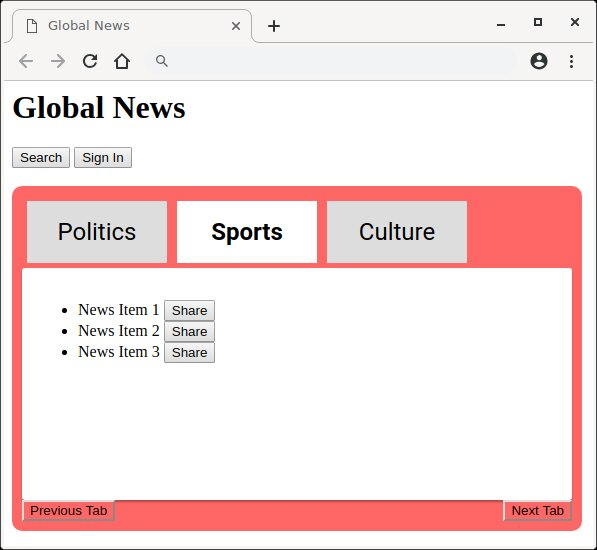
\includegraphics[width=\linewidth]{fancytabs-normal}
    \end{minipage}
  \end{lrbox}
  \begin{lrbox}{\sndlst}%
    \begin{minipage}{.63\linewidth}
      \begin{html}[basicstyle=\ttfamily\scriptsize]
<fancy-tabs>
  <button slot="title">Politics</button>
  <button slot="title" selected>Sports</button>
  <button slot="title">Culture</button>
  <section>content panel 1</section>
  <ul>
    <li>News Item 1 <button>Share</button></li>
    <li>News Item 2 <button>Share</button></li>
    <li>News Item 3 <button>Share</button></li>
  </ul>
  <section>content panel 3</section>
</fancy-tabs>
      \end{html}
    \end{minipage}
  \end{lrbox}
  \subfloat[\label{fig:running-example-user}
    User view
  ]{\usebox{\fstlst}}%
  \hfill%
  \subfloat[\label{fig:running-example-consumer}
    Consumer view
  ]{\usebox{\sndlst}}
  \caption{A simple example: a fancy tab component.}\label{fig:running-example}
\end{figure}

The left-hand side of \autoref{fig:running-example} shows the rendered
output of the widget in use while the right-hand side shows the HTML
source code snippet.  It provides a custom HTML tag
\inlinehtml{<fancy-tabs>} using an HTML template that developers can
use to include the widget. Its children will be rendered inside the
widget, more precisely, inside its \emph{slots} (elements of type
\inlinehtml{slot}).  It has a slot called ``title'' and a default
slot, which receives all children that do not specify a ``slot''
attribute.

It is important to understand that slotting does \emph{not change} the
structure of the DOM (\ie, the underlying pointer graph): instead,
slotting is implemented using special element attributes such as
``slot,'' which control the final rendering. The DOM standard
specifies methods that inspect the effect of these attributes such as
\texttt{assigned\_slot}, but the majority of DOM methods do not
consider the semantics of these attributes and therefore do not
traverse into shadow trees.

This provides an important boundary for client-side code. For example,
a JavaScript program coming from the widget developer that changes the
style attributes of the ``Previous Tab'' and ``Next Tab'' buttons in the lower
corners of the widget will not affect buttons belonging to other parts
coming from outside, \ie, the application of the widget consumer.
Similarly, a JavaScript program that changes the styles of buttons
outside of Fancy Tab, such as the navigation buttons, will not have
any effect on them, even in the case of duplicate identifiers.

Sadly, the DOM standard neither defines the concept of web components
nor specifies the safety properties that they should guarantee, not
even informally. Consequently, the standard also does not discuss how
or even if the methods for modifying the node tree respect component
boundaries.  Thus, shadow roots are only the very first step in
defining a safe web component model.

Earlier~\cite{brucker.ea:core-dom:2018,brucker.ea:afp-core-dom:2018},
we presented a formalization of the ``flat'' DOM (called Core DOM)
without any support for shadow trees or components.  We then extended
this formalisation with support for shadow trees and
slots~\cite{brucker.ea:afp-shadow-dom:2020}.

In this AFP entries, we use the basis provided by our earlier work for
defining a \emph{formally verified model of web components} in general
and, in particular, the notion of \emph{weak} and \emph{strong
  component safety}. For all methods that query, modify, or transform
the DOM, we formally analyze their level of component safety. In more
detail, the contribution of this AFP entry is four-fold:
\begin{enumerate}
\item We provide a formal model of web components and their safety
  guarantees to web developers, enabling a compositional development
  of web applications,
\item for each method, we formally verify that it is either weakly or
  strongly component safe, or we provide a proof showing
  that it is not component safe,
\item we fill the gaps in the standard by explicitly formalizing
  invariants that are left out in the standard. These invariants are
  required to ensure that methods in the standard preserve a valid
  node tree. Finally,
\item we present a formal model of the DOM with shadow roots including
  the methods for querying, modifying, and transforming DOM instances
  with shadow roots.
\end{enumerate}
Overall, our work gives web developers the guarantee that their code
will respect the component boundaries as long as they abstain from or
are careful when using certain DOM methods such as
\texttt{appendChild} or \texttt{ownerDocument}.

The rest of this document is automatically generated from the
formalization in Isabelle/HOL, i.e., all content is checked by
Isabelle (we refer readers interested in a more high-level
presentation of the work to \cite{herzberg:web-components:2020,
  brucker.ea:web-components:2019}. The structure follows the theory
dependencies (see \autoref{fig:session-graph}).

\begin{figure}
  \centering
  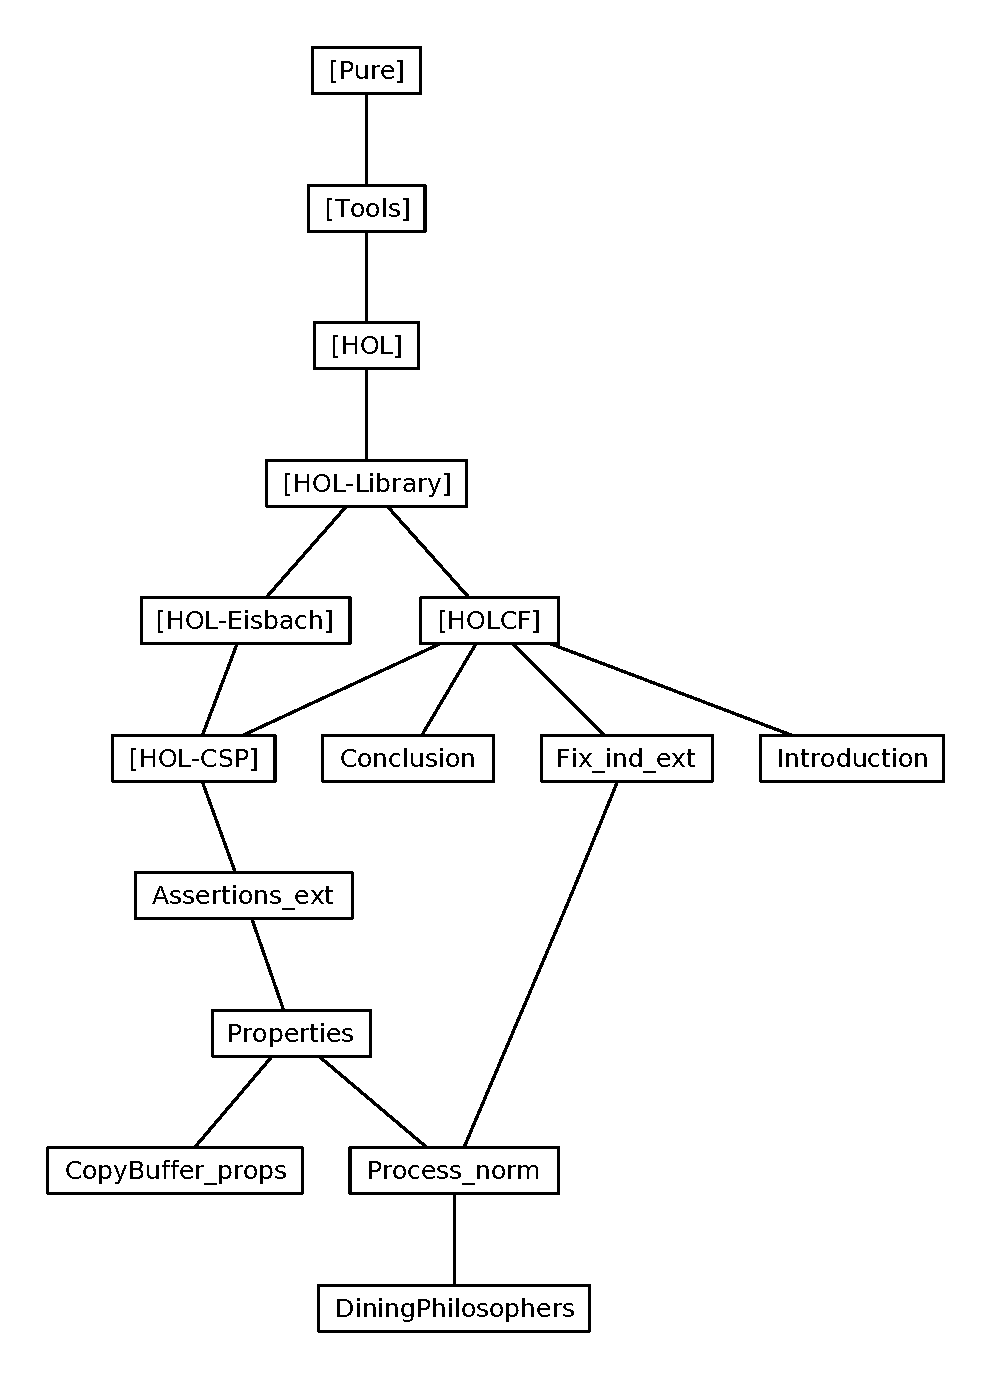
\includegraphics[width=.8\textwidth]{session_graph}
  \caption{The Dependency Graph of the Isabelle Theories.\label{fig:session-graph}}
\end{figure}

\clearpage

\chapter{Web Components}
\label{cha:components}
\input{Core_DOM_Components.tex}
\input{Shadow_DOM_Components.tex}

\chapter{Example}
\label{cha:example}
\input{fancy_tabs.tex}

{\small
  \bibliographystyle{abbrvnat}
  \bibliography{root}
}
\end{document}

%%% Local Variables:
%%% mode: latex
%%% TeX-master: t
%%% End:
